\documentclass[conference]{acm_proc}

\usepackage{epsfig,endnotes}
\usepackage{xspace}
\usepackage{array}
\usepackage{graphicx,algorithm,algorithmic,xspace,subfigure,color,url,multirow,listings,booktabs}
\usepackage{pdfsync, caption}
\usepackage{balance}
%our commands
%\usepackage{setspace}
%\doublespacing

\usepackage{url}

\newcommand{\delete}[1]{}
\newcommand{\tfs}{TableFS\xspace}
\newcommand{\giga}{GIGA+\xspace}
\newcommand{\ldb}{{LevelDB}\xspace}
\newcommand{\comment}[1]{{\color{red} [{#1}]}}
\newcommand{\kai}[1]{\comment{Kai says: #1}}

%\hyphenation{op-tical net-works semi-conduc-tor}

\begin{document}

%don't want date printed
\date{}

%make title bold and 14 pt font (Latex default is non-bold, 16 pt)
\title{Building a High-Performance Metadata Service by Reusing Scalable I/O Bandwidth}

\numberofauthors{1}

\author{
\alignauthor
Kai Ren, Swapnil Patil, Kartik Kulkarni, Adit Madan, Garth Gibson \\
\affaddr{Carnegie Mellon University}\\
\email{\{kair, svp\}@cs.cmu.edu, \{kartikku, aditm\}@andrew.cmu.edu, garth@cs.cmu.edu}
}

\maketitle

\begin{abstract}
Modern parallel and cluster file systems provide highly scalable I/O bandwidth
by enabling highly parallel access to file data.
Unfortunately metadata access does not benefit from parallel data transfer,
so metadata performance scaling is less common.
To support metadata-intensive workloads,
we offer a middleware design that layers on top of existing cluster
file systems, adds support for load balanced and
high-performance metadata operations without sacrificing data bandwidth.
We proposed and compared several distributed indexing mechanisms
with trade-offs on performance of different file system operations,
along with optimized log-structured metadata on-disk representation.
The integration requires several optimizations including cross-server split
operations with minimum data migration, and decoupling of
data and metadata paths.
We implement and deploy our metadata middleware on a 256-node
cluster and demonstrate its almost linear scalability, and
its out-of-core metadata performance comparable
to Hadoop HDFS's pure in-memory solution on a single server.

\end{abstract}
\section{Introduction}

% Explain what is file system metadata

% What is the current bottleneck

% Why do comparative study

% What is the contribution?



\section{System Design and Implementation}

\begin{figure}[!hb]   %% START_FIGURE
\centerline{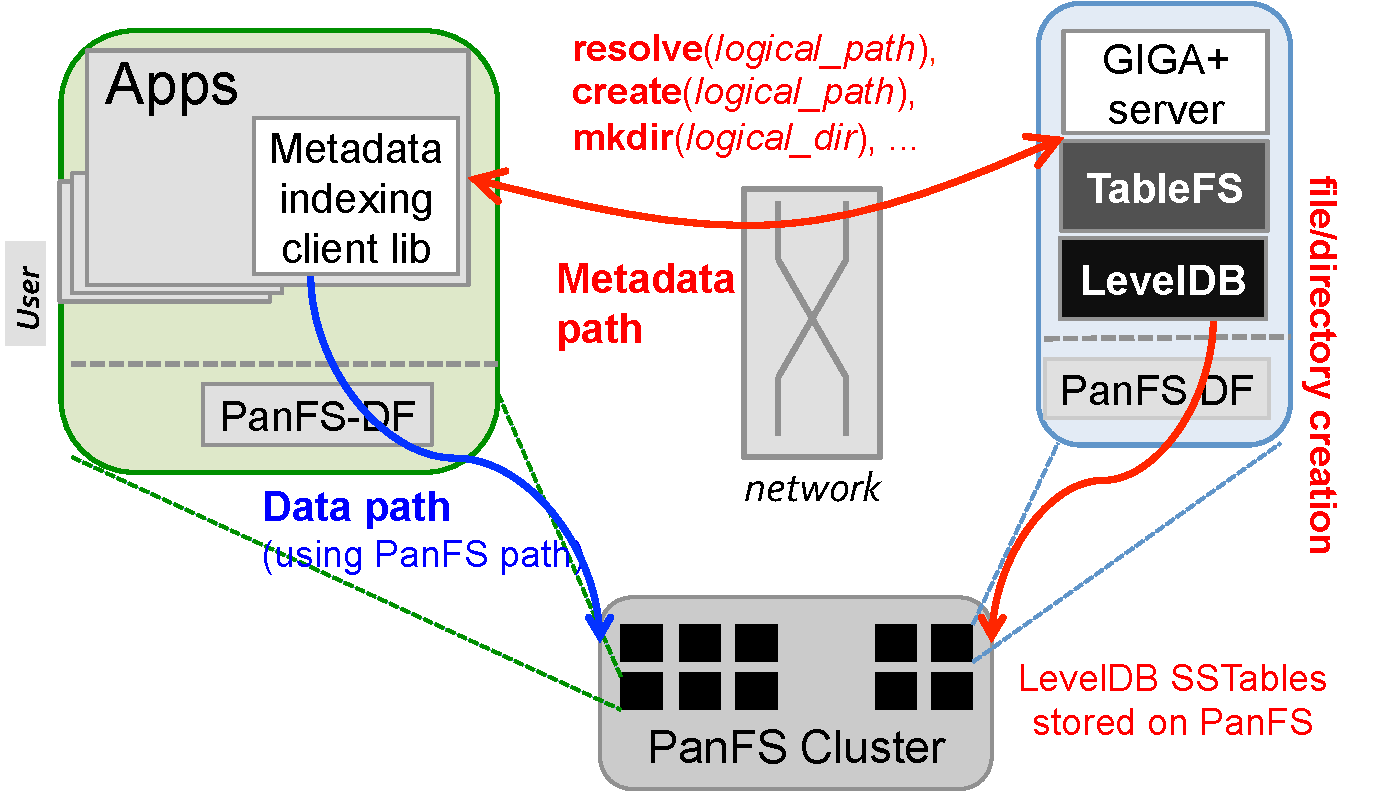
\includegraphics[scale=0.35]{./figs/giga-impl-leveldb-clusterfs}}
\vspace{10pt}
\caption{\textit{\footnotesize
The metadata servers deploys different policies to partition metadata
over multiple servers, and uses an Log-Structured Merge tree (LevelDB)
to manage out-of-core metadata representation on disk.
This integrated solution is layered on top of an existing distributed
file system deployment (e.g. HDFS) to improve its metadata and
small file operation efficiency.
}}
%\vspace{10pt}
\hrule
\label{fig:design}
\end{figure}       %% END_FIGURE

Figure \ref{fig:design} presents the overall architecture of our scalable
metadata service. Our metadata service is a middleware inserted into
existing deployments of distributed file systems to improve metadata efficiency
while maintaining high I/O bandwidth for data transfers.
The system uses a client-server architecture,
and consists of three core components:

\begin{itemize}
\item{\textbf{Client:}} Applications interact with our middleware
through a library directly linked into the application,
(or through the FUSE user-level file system \cite{fuse}).
The stateless client-side code redirects applications' file operations
to the appropriate destination according to the types of operations.
All metadata requests (e.g. \texttt{create()} and \texttt{mkdir()}),
and data requests on small files (e.g. \texttt{read()} and \texttt{write()}),
are handled by the metadata indexing modules that address
these requests to the appropriate server.
For all data operations on large size files, the client code redirects
the request directly to the underlying distributed file system to take full
advantage of data I/O bandwidth. A newly created, but growing file
may be transparently reopened by the client module.

\item{\textbf{Metadata Indexing Server:}}
Each indexing server manages its local metadata storage backend to store and
access all metadata information and small file data.
It can plug-in different indexing policies to
partition large directories across indexing servers.
It also monitors the growth of small files,
and migrates newly large files into the underlying distributed file system
when its size exceeds a threshold.

\item{\textbf{Metadata Storage Backend:}}
The metadata storage backend packs metadata and small file data into
large, log-structured, flat files, and stores these files
in the underlying distributed file system.
It uses a modified version of LevelDB \cite{leveldb} that
converts random updates into sequential writes, and improves disk performance.
In order to dynamically redistribute large directories,
the metadata storage backend also modifies LevelDB
to support exporting and importing a large list of key-value pairs in batch.

\end{itemize}

Remainder of this section describes more details of our system.
Section \ref{design.leveldb} shows how our metadata service
stores all file system metadata and small files
using a single on-disk structure on each server.
Section \ref{design.decouple} focus on the challenges in effectively
integrating our metadata middleware service with the underlying
distributed file systems. The rest sections discuss
distributed transaction support and fault tolerance strategy.

\subsection{Metadata Storage Backend}
\label{design.leveldb}

Our metadata storage backend implements a modified version of LevelDB
\cite{leveldb} to pack together and manage all the metadata and small files,
hiding them from the underlying cluster file system.
LevelDB is an open-source implementation of an Log-structure Merge (LSM) tree \cite{ONeil1996},
which provides a simple key-value store interface,
supporting point queries and range queries. In LevelDB, by default,
a set of changes are spilled to disk when the total size of modified
entries exceeds 4 MB.  When a spill is triggered,
the changed entries are sorted, indexed and written to disk
as an immutable file called an SSTable \cite{BigTable}.
These entries may then be discarded from the in memory buffer.
Discarded entries can be reloaded by searching each SSTable on disk,
possibly stopping when the first match occurs if the SSTables are
searched most recent to oldest.  The number of SSTables that need to be
searched is reduced by maintaining the minimum and maximum key value
and a Bloom filter\cite{bloomfilter} on each,
but, with time, the cost of finding a record not in memory still increases.
Compaction is the process of combining multiple overlapping range SSTables
into a number of disjoint range SSTables by merge sort.
More details about LevelDB can be found in its website \cite{leveldb}.

~\\
\textbf{Metadata representation: }
LevelDB aggregates directory entries,
inode attributes and small files into one LSM tree
with an entry for each file and directory.
To translate the hierarchical structure of the file system namespace
into key-value pairs, the 224-bit key is chosen to consist of
the 64-bit i-node number of a entry's parent directory
and a 160-bit SHA-1 hash value of its filename string
(final component of its pathname) as shown below:

\begin{table}[!htc]
\center
\vspace{10pt}
\begin{tabular}{c|c}
key & \texttt{Parent directory ID, hash(Object name)} \\
\midrule
value & \texttt{Attributes,[Symbolic link|Data]} \\
\end{tabular}
\label{tab:keyschema}
\end{table}

The value of an entry contains the file's full name and i-node attributes,
such as i-node number, ownership, access mode, file size, timestamps (\textit{struct stat} in Linux).
For small files with size less than $T$ (defaulting to 4KB),
the value field also contains the file's data.
For large files, the file data field in a file row of the table
is replaced by a symbolic link that points to
the actual file object in the underlying file system.
LevelDB also preserve additional information for different
indexing policy. For dynamic namespace partition,
it also records hash partition related mapping information for directories
used in \giga.

~\\
\textbf{Partition splitting: }
To effectively build indexing server that integrates
the dynamic namespace distribution mechanism
and our on-disk metadata representation,
we have to modify LevelDB to support for
migrating directory partitions as required by \giga.

The file system metadata, including \giga directory partitions and their directory
entries are stored in \ldb as a set of immutable files (SSTable files)
in a server specific directory in the underlying distributed file system.
Each metadata indexing server process splits a large partition $P$ on
into itself and another hash partition $P'$ which is managed by a
different server; this split involves migrating approximately half the entries
from old partition $P$ to the new partition $P'$ on another server.
During splitting, the partition in migration is locked against client
for simplification. We explored several ways
to perform this cross-server partition split.

A straightforward solution would be to perform a range scan on
partition $P$, and remove about half the entries
(that will be migrated to the new partition $P'$) from $P$.
All removed entries would then be batched together
and sent in a large RPC message to the server that will manage partition $P'$.
The split receiver would insert each key in the batch into its own \ldb instance.
While simplicity of this solution makes it attractive,
it is slow in practice and vulnerable to failures during splitting.

We have devised a faster and safer technique to
reduce the time that the splitting range is locked.
The immutability of SSTables in \ldb makes a fast bulk insert possible --
an SSTable whose range does not overlap any part of a current LSM tree
can be added to Level 0 without its data being pushed through the
write-ahead log and minor compaction process.
To take advantage of this opportunity, we extended \ldb
to support a three-phase \giga split operation:

\begin{itemize}
\item{Phase 1:} The split initiator locks and
then performs a range scan on its \ldb instance
to find all entries in the hash-range that needs to be moved to another server.
Instead of packing these into an RPC message,
the results of this scan are written in SSTable format to a file in the
underlying distributed file system.

\item{Phase 2:} The split initiator notifies the split receiver about
the path to the SSTable-format split file in a much smaller RPC message.
Since this file is stored in shared storage,
the split receiver directly inserts this file as a symbolic link
into the \ldb tree structure without actually copying this file.
The insertion of this file into the split receiver is the commit
part of the split transaction.

\item{Phase 3:} The final step is a clean-up phase:
after the split receiver completes the bulk insert operation, it notifies the
initiator, who then deletes the migrated key-range from its \ldb instance
and unlocks the range.
\end{itemize}


\subsection{Decoupled Data and Metadata Path}
\label{design.decouple}

\subsection{Transaction Support}

\subsection{Fault Tolerance}


\section{Experimental Evaluation}

This section evaluates the scale and performance of \sys using a mix of
metadata-intensive and data-intensive benchmarks. Our evaluation layers \sys on
the Panasas PanFS file system, and focuses on three questions:
\begin{itemize}
\item How does \sys enhance metadata throughput, particularly
number of file creates per second for concurrent file creation workloads, on
the PanFS storage system?
\item What is the data throughput of \sys layered on PanFS for N-N checkpointing 
workload found in HPC systems?
\item How portable is \sys to be used on other cluster storage systems and
configurations?
\end{itemize}

\subsection{Setup and methodology}

Our prototype is implemented in about 14,000 lines of C code using
a modular design comprising of \tfs, \ldb and PanFS layers. In particular, the
PanFS layer is unmodified and can be replaced with any other cluster file
system. The current version implements most common POSIX file system operations 
except \texttt{hardlink}, \texttt{rename}, and \texttt{xattr} related operations.
The first two operations, \texttt{hardlink} and \texttt{rename}, are
particularly complicated because they need distributed transaction support for
correct and fault tolerant cross-server operations; this problem is beyond the
scope of this paper.

All experiments were performed on two clusters described in Table
\ref{tab:setting}. The first cluster is a 5-shelf PanFS storage cluster, and the 
second cluster is a 64-node setup to run \sys code and applications.
Table \ref{tab:setting} describes the hardware and software configuration of
these clusters.
The first cluster is used to evaluate the scale and performance of the
underlying cluster file system that uses our middleware.
The second cluster is used to demonstrate that our middleware 
solution can be layered on other file system deployments without any
configuration changes; this setup
emulates a case that each GIGA+ server runs in a different NFS node and manages 
its own \tfs instance locally to scale the metadata performance of NFS.
In all tests, the client uses library version code;
the threshold for splitting a partition is always 8,000 entries;
and \tfs managed by GIGA+ server syncs its data every 5 seconds.

\begin{footnotesize}
\begin{table}
\begin{tabular}{lcc}
\toprule
      & Cluster 1 & Cluster 2 \\
      & (Storage cluster) & (Test applications)\\
\midrule
\#Nodes & 5 & 64 \\
\hline
OS &   CentOS 6.3 &  Ubuntu 12.10 \\
Kernel & 2.6.32 x86\_64 & 3.6.6 x86\_64 \\
\hline
CPU & AMD Opteron 6272 &  AMD Opteron 242 \\
    & 64 Cores & Dual Core\\
\hline
Memory & 128GB DDR &  16GB DDR \\
\hline
Network & 40GE NIC &  1GE NIC  \\
\hline
Storage & PanFS & Western Digital \\
System &      5 Shelves & Local hard disk  \\
       &   (5 MDS + 50 ODS) &  2TB per node  \\
\hline
& & 100 seeks/sec \\
& & random seeks   \\
& & 137.6 MB/sec  \\
& & seq. reads    \\
& & 135.4 MB/sec  \\
& & seq. writes   \\
\bottomrule \\
\end{tabular}
\caption{
\textit{\footnotesize Settings of two clusters used for evaluation.}
}
\label{tab:setting}
\end{table}
\end{footnotesize}

In the following sections, we will first show the evaluation
on the end-to-end performance of the integrated system on top of PanFS,
and then present the results of a strong scaling experiment on another platform.

\subsection{Full system evaluation}
\label{sec:fullsystem}
We performed an end-to-end evaluation of our prototype in a cluster with 5 test nodes.
The cluster is connected to a 5-shelves PanFS storage system
with 5 metadata nodes and 50 storage nodes.
Since each test node has 64 cores and a 40GE NIC, they are able to
to saturate the data bandwidth of our PanFS storage cluster.
Because of some technique difficulties,
we did not run our GIGA+ server processes inside the metadata node.
Instead, we co-locate our GIGA+ server processes
with client processes in the test nodes.
Each test node runs a GIGA+ server that is assigned to a metadata node
as explained in Section \ref{design.integration}.
We ran a series of HPC benchmarks (used by parallel file system vendors and users)
to test metadata path and data path separately,
including the open source \textit{mdtest} synthetic benchmark \cite{mdtest}
and File System Test Suite checkpoint benchmark from LANL \cite{mpiio}

\textbf{Metadata Intensive Workloads -- }
We used the synthetic mdtest benchmark \cite{mdtest}
to generate a three-phase workload:
The first phase is to create 5 million
zero-files in a single shared directory \cite{ceph:weil06, GIGA11};
the second phase is to perform $stat()$ on random files in the directory;
the third phase is to delete all the files in the directory in a random order.
Each phase involves multiple clients to issue the operations concurrently.

If we directly use the above workload to directly compare our layered system
against the original PanFS, it would not be fair enough.
This is because a single directory can only use the hardware resource
of one metadata manager in PanFS,
and PanFS also limits a single directory to 1 million files.
Therefore we chose to compare native PanFS creating 1 million files
in 5 different directories owned by 5 different metadata managers.
The total number of clients used for testing the two systems
are kept the same.

\begin{figure}[t]  %%%%%%%%%%%%%%%%%%%%%%%
\centerline{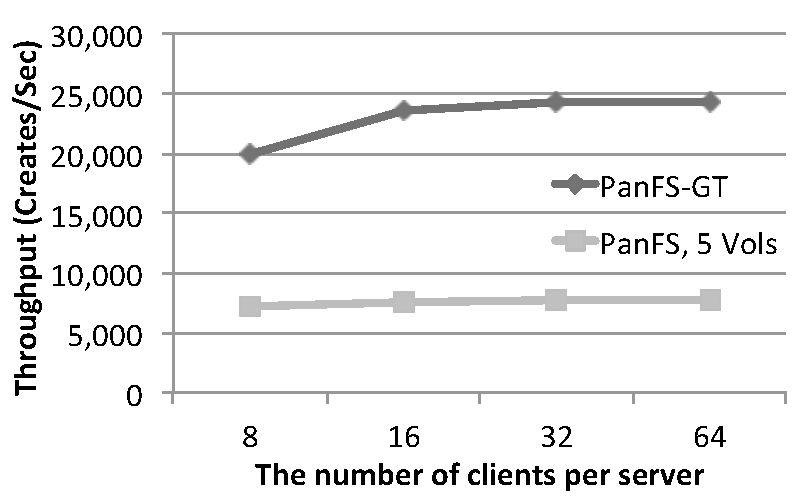
\includegraphics[scale=0.7]{./figs/zero_file_creation_on_panfs}}
\vspace{10pt}
\caption{\normalsize
\textit{Average throughput during creating five million zero-length files
in one empty directory with different number of clients per test node.
Running 32 and more clients per test node is able to saturate \sys
and original PanFS}
}
\vspace{10pt}
\hrule
\label{graph:creation_clients}
\end{figure}       %%%%%%%%%%%%%%%%%%%%%%%

\begin{figure}[t]  %%%%%%%%%%%%%%%%%%%%%%%
\centerline{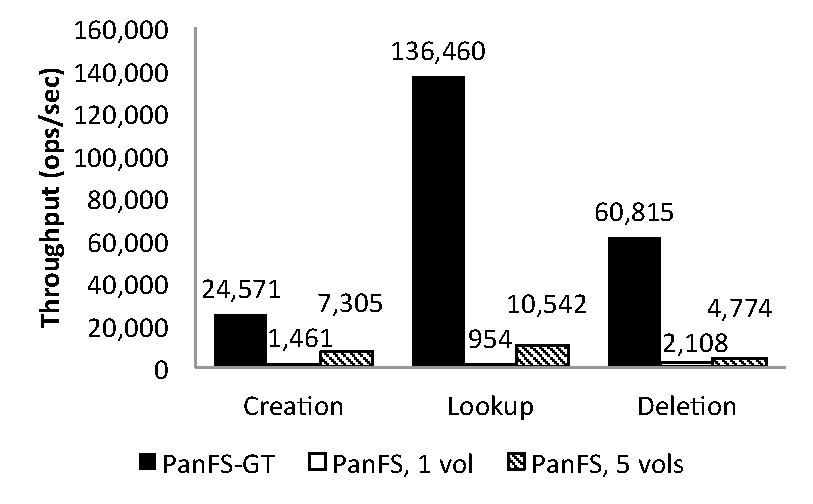
\includegraphics[scale=0.7]{./figs/mdtest}}
\vspace{10pt}
\caption{\normalsize
\textit{mdtest:
The average aggregated throughput of different operations in mdtest
when generating 5 million zero-length files in a single shared directory.
Since PanFS has a hard limit to allow only create 1 million entries
in one directory, the bar showing PanFS with 1 volume only gives
the average throughput for the case of creating 1 million entries.
}
}
\vspace{10pt}
\hrule
\label{graph:mdtest_ops}
\end{figure}       %%%%%%%%%%%%%%%%%%%%%%%


Figure \ref{graph:creation_clients} shows the aggregated througphut during
the first phase. We varies the nubmer of clients running in each test node
to find the right number that can saturate both systems.
Both systems achieve the highest aggregated throughput when the number
of clients per node is 32 or more. In all the experiments shown later,
we present the results with 32 clients per test node if without explanation.
For all cases, \sys  is approximately 3.5 times faster than the native PanFS
using 5 volumes. The aggregated throughput with 32 clients per server
achieves about 24,571 creation per second.

Figure \ref{graph:mdtest_ops} shows the aggregated througphut of
different operations during three phases in mdtest.
Besides \sys and PanFS using 5 volumes, it also shows
the aggregated throughput of creating 1 million files in one volume of PanFS.
For $lookup$ and $deletion$ workloads,
\sys gains more advantages over original PanFS,
and achieves about 10 to 15 times speed up.
Fast lookup is due to the memory indexing and Bloom filters in \ldb.
For deletion of a key, \ldb essentially just inserts the key and a deletion mark
into its memtable, and delays the actual deletion in later compaction processes.


\textbf{Small File Workloads -- }
We also use mdtest benchmark to generate files with small size data to evaluate
the effectiveness of embedding file content with the metadata inside \tfs.
Similar to the previous test,
mdtest benchmark creates 5 million files in a single directory
but with file data of two different sizes: 4KB and 16 KB.
4KB is the median file size for many desktop workloads \cite{Bill11},
and 16KB is the median file size for some large storage clusters using PanFS \cite{brent13}.
The threshold $T$ for our prototype is set to 64KB, so all these files
are stored in \tfs instance.

%compaction and CPU usage
Figure \ref{graph:smallfiles} shows the aggregated throughput during the test,
which is aggregated from all clients. For 4KB file size,
\sys is about $2.5\times$ faster than original PanFS.
However, \sys is about $35\%$ slower than PanFS for 16KB file size.
We found that embedding 16KB file makes the key-value pair significanly larger,
and causes higher write amplification during compaction process in \ldb,
since \ldb tries to merge sort both file data and metadata.
Additionally, \ldb will firstly write the inserted key-value pairs
to the transaction log, and then (during a compaction) to the SSTable.
With larger key-value pairs, LevelDB's per-operation efficiency is
slowed down by the cost of extra copies of large values.
This suggests that the threshold $T$ for embedding file size should not be
greater than 16 KB. For larger embedding file size,
we might sacrafice the read performance to maitain its fast insertion rate
by using column-based approach which stores metadata and small file separately.
Such investigation is left for future works.

\begin{figure}[t]  %%%%%%%%%%%%%%%%%%%%%%%
\centerline{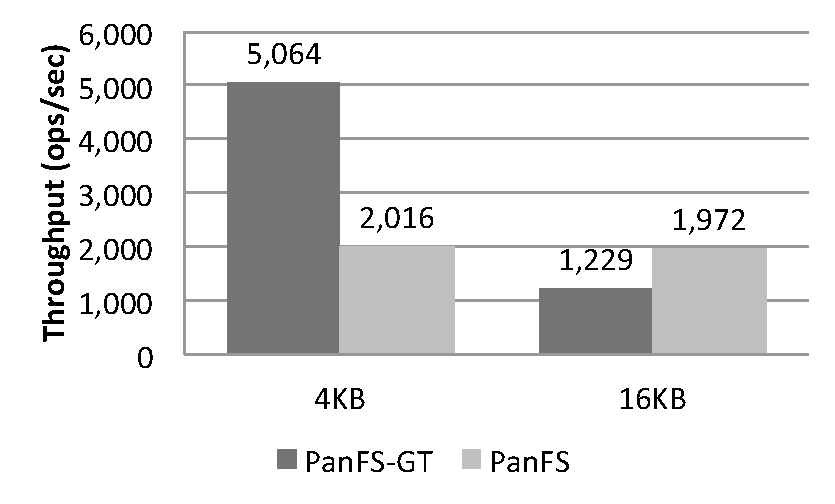
\includegraphics[scale=0.7]{./figs/small_file_creates}}
\vspace{10pt}
\caption{\normalsize
\textit{Average aggregated throughput during creating 5 million small files
with different size in one shared directory}
}
\vspace{10pt}
\hrule
\label{graph:smallfiles}
\end{figure}       %%%%%%%%%%%%%%%%%%%%%%%


%Library version not FUSE
%Clean cache

\textbf{Data Intensive Workloads -- }
The LANL filesystem checkpoint benchmark can
generate many types for HPC checkpoint I/O patterns.
For our test purposes, we configured the benchmark to generate
a concurrent N-N checkpoint write and read workload.

All checkpoint file I/O is performed by a set of processes
that synchronize with each other using MPI barriers.
At the begining, each process opens a freshly created checkpoint file
for writing and then waits at a barrier until all processes are ready to write.
Once all processes are ready, each processes starts
concurrently writing the checkpoint data to its own file,
until it has written the specified number of bytes.
It then waits barrier for all the other processes to finish writing,
and finally syncs its data to the file system and closes the file.
Before starting the read phase we terminate all processes
accessing these checkpoint files so that
we can unmount the filesystem in order to ensure that
all freshly written data has been flushed out from all the nodes' memory
to prevent caching from unfairly biasing our read performance.
After the filesystem has been mounted and restarted,
the benchmark reads the checkpoint in the same way it was written,
however we shift, so each process will read
the file generated by another process.

In this test, we also vary the number of clients per test node
from 8 to 64 clients. The clients in each node will generate
640GB checkpoint data in total to the underlying file system,
no mater what number of clients each node has.
The size of data buffer for each file system call is set to be 16KB.
For \sys, the checkpoint files generated in the test will be
first stored in \tfs, and the migrated to the underlying PanFS.

Figure \ref{graph:checkpoint_write} and \ref{graph:checkpoint_read}
show the average throughput during the write phase and read phase
in the N-N checkpoint workload respectively. We can see \sys
performs comparably with the native PanFS.
For read checkpoint worload, the largest performance loss is less than $10\%$.
And \sys is even faster in write checkpoint phase.
The embedding of small files do not affect the data transferring
of large files.

\begin{figure}[t]  %%%%%%%%%%%%%%%%%%%%%%%
\centerline{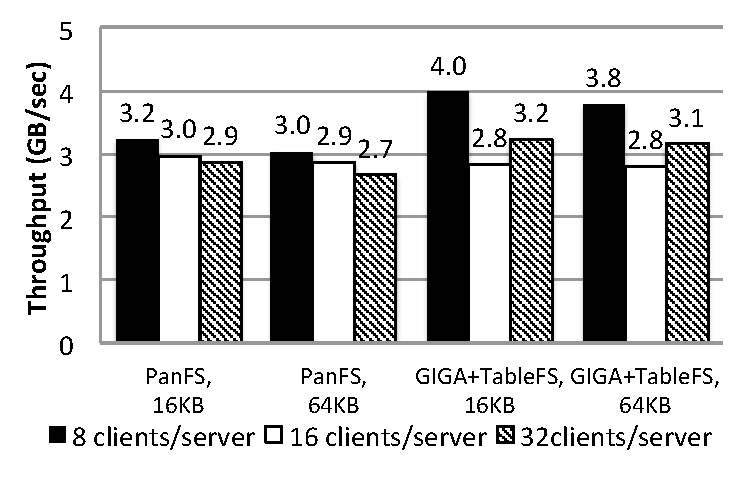
\includegraphics[scale=0.7]{./figs/checkpointing_write}}
\vspace{10pt}
\caption{\normalsize
\textit{
The aggregated write throughput in N-N check-pointing workload.
Each volume receives 640 GB data.
}
}
\vspace{10pt}
\hrule
\label{graph:checkpoint_write}
\end{figure}       %%%%%%%%%%%%%%%%%%%%%%%

\begin{figure}[t]  %%%%%%%%%%%%%%%%%%%%%%%
\centerline{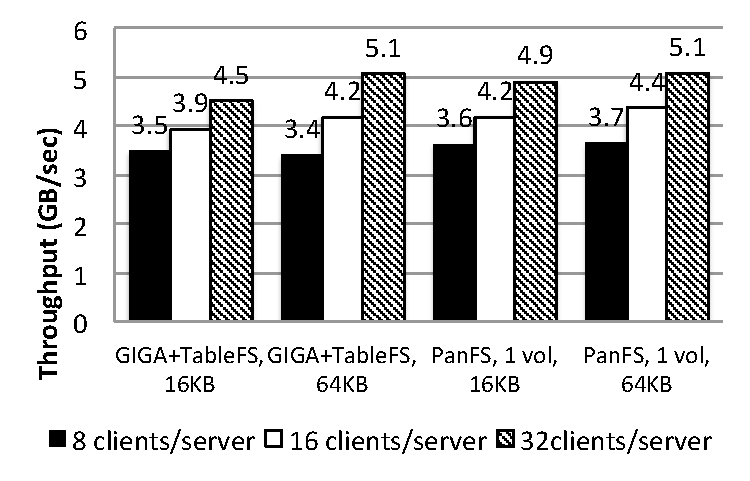
\includegraphics[scale=0.7]{./figs/checkpointing_read}}
\vspace{10pt}
\caption{\normalsize
\textit{
The aggregated read throughput in N-N check-pointing workload.
}
}
\vspace{10pt}
\hrule
\label{graph:checkpoint_read}
\end{figure}       %%%%%%%%%%%%%%%%%%%%%%%



\subsection{Evaluating scaling behavior}

\begin{figure*}[t]
\centerline{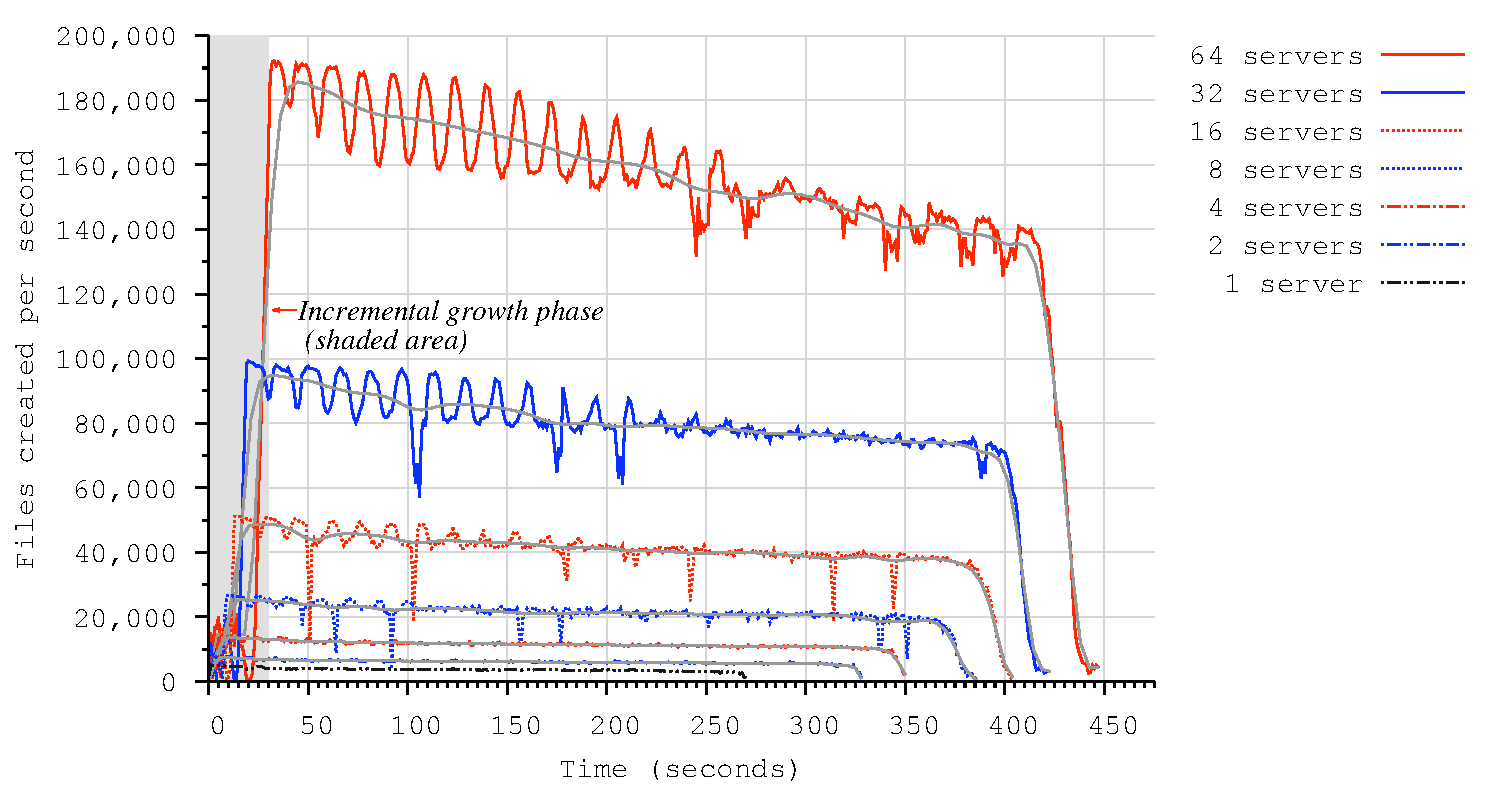
\includegraphics[scale=0.55]{./figs/ldb_insertrate}}
\vspace{10pt}
\caption{\textit{\footnotesize 
Our middleware metadata service prototype shows promising scalability
up to 64 servers.
Note that at the end of the experiment,
the throughput drops to zero
because clients stop creating files as they finish 1 million files per client.
(Solid lines are Bezier curves to smooth the variability.)
}
}
%\vspace{10pt}
\hrule
\label{graph:ldb-scaling}
\end{figure*}

This section shows how \sys scales over time in large multi-server setup. To
understand this behavior we layered \sys on a different cluster (cluster \#2
from Table \ref{tab:setting}) comprising of 64-nodes running \sys clients and
servers. The main difference is the backend storage: this analysis emulates a
federated NFS setup where each \psys server process in node manages its own \tfs 
instance and store SSTables into a local disk.
To emulate shared storage for split operations, we used a NFS-mounted shared 
directory accessible from all machines; this shared directory was only used for 
moving SSTables of splitting directory partitions across servers.
%The distributed logging is not available in this experiment setting,
%but which does not limit testing the scalability of our system.

This analysis uses a \textit{strong scaling} experiment that creates
1 million files per server, for a total of 64 million files in the
64-server configuration. We vary the number of servers from 1 to 64
to understand how performance scales with more servers.

Figure \ref{graph:ldb-scaling} shows the instantaneous throughput
during the concurrent create workload.
The main result in this figure is that as the number of servers doubles the
throughput of the system also scales up. With 64 servers, \giga can achieve a
peak throughput of about 190,000 file creates per second.
The prototype delivers peak performance after the directory workload
has been spread among all servers.
Reaching steady-state, the throughput quickly grows
due to the splitting policies adopted by \giga.


After reaching the steady state, throughput slowly drops
as \tfs builds a larger metadata store.
In fact, in large setups with 8 or more servers,
the peak throughput drops by as much as 25\% (in case of the 64-server setup).
This is because when there are more entries already existing in \tfs,
it requires more compaction work to maintain invariants inside \ldb
and to perform a negative lookup before each create
has to search more SSTables on disk.
In theory, the work of inserting a new entry to a LSM-tree is $O(\log_{B}(n))$
where $n$ is the total number of inserted entries, and $B$ is a constant factor
proportional to the average number of entries transferred in each disk request
\cite{Bender2007}.
Thus we can use the formula $\frac{a\cdot S+b}{\log{T}}$ to
approximate the throughput timeline in Figure \ref{graph:ldb-scaling},
where $S$ is the number of servers, $T$ is the running time,
and $a$ as well as $b$ are constant factors
relative to the disk speed and splitting overhead.
This estimation projects that when inserting 64 billion files with 64 servers,
the system may deliver an average of 1,000 operations per second per server,
i.e. 64,000 operations per second in aggregate.
This still exceeds today supercomputer's most rigorous scalability demands for
40,000 file creates per second in a single directory \cite{hpcs-io:2008}.


\section{Related Work}
\label{relatedwork}

This paper proposes a layered approach that allows a cluster file system to 
distribute both namespace and directories. In this section, we discuss prior
work related to metadata systems in modern cluster file systems and optimized
layouts for high-performance metadata.

In many cluster file systems, the metadata path lacks the concurrency and 
scalability found in the data path.
Many file systems, including Lustre \cite{lustre}, Google file system
\cite{gfs:ghemawat03} and HDFS \cite{HDFS}, continue to rely on a single
metadata server to store all file system metadata. This simplifies the
complexity of administration and implementation, but limits the scalability to 
how fast one server can service all metadata operations. 
Some cluster file systems distribute metadata on multiple metadata servers. The 
main difference is what metadata is distributed and how it is distributed.

PanFS and PVFS cluster distribute different parts of the namespace on different
metadata servers.
PanFS uses a coarse-grained distribution by assigning a subtree of the
namespace (called volume) to each metadata server (called directory blade) 
\cite{panfs:welch08}.
PVFS is more fine-grained: it spreads different directories, even the ones in
the same sub-tree, on different metadata servers \cite{pvfs}.
However, both PanFS and PVFS lack support for distributed directories.

Few cluster file systems have added support for distributed directories but
each system uses a different technique to spread these directories.
A beta release of OrangeFS, a commercially supported PVFS distribution, uses a 
simplified version of GIGA+ to distribute large directories on several metadata 
servers \cite{OrangeFS}.
Ceph uses an adaptive partitioning technique called CRUSH for distributing its
metadata and directories on multiple metadata servers \cite{ceph:weil06}. While
experimental version of Ceph (from 2006) shows promising directory scalability,
the recent versions of Ceph directory clustering have been described as
"less stable" \cite{ceph-baddirs1:www} and "buggy" \cite{ceph-baddirs2:www}.
IBM GPFS uses extensible hashing to distribute directories on different disks on 
a shared disk subsystem \cite{gpfs:schmuck02}. GPFS has the most complete and
stable distributed directory implementation, but its design relies heavily on
cache consistency and distributed locking mechanisms. When compared to GIGA+,
this may result is much lower file create performance (when files are created
in a single directory) but GPFS delivers very high directory read performance 
by caching directory blocks on all readers \cite{GIGA11}.

The second aspect of this paper is the use of a optimized single-node metadata
representation that enables high throughput (metadata operations per second).
Several recent efforts have focused on using advanced data-structures, such
as modified LSM-trees, stratified B-trees and fractal trees, to speed up number
of IOs per second \cite{blsm, tokufs, Andrew11}. 


\section{Conclusion}
\label{conclusion}


%\section*{Acknowledgment}
%This research is supported in part by The Gordon and Betty Moore Foundation, NSF under award, SCI-0430781 and
%CCF-1019104, Qatar National Research Foundation 09-1116-1-172, DOE/Los Alamos National Laboratory, under contract number DE-AC52-
%06NA25396/161465-1, by Intel as part of the Intel Science and Technology Center for Cloud Computing (ISTC-CC), by gifts from
%Actifio, EMC, Emulex, Facebook, Fusion-IO, Google, Hewlett-Packard, Hitachi, Huawei, Intel,
%NEC, NetApp, Oracle, Panasas, Samsung, Seagate, STEC, Symantec, VMWare, and Western Digital.
%We thank the member companies of the PDL Consortium for their interest, insights, feedback, and support.

\bibliographystyle{plain}
\bibliography{reference}

\end{document}
